\section*{
ماشین حالت
\LTRfootnote{State Machine}
}
حالات ماشین حالت را می‌توانید در شکل زیر مشاهده نمایید:
\begin{figure}[H]
	\centering
	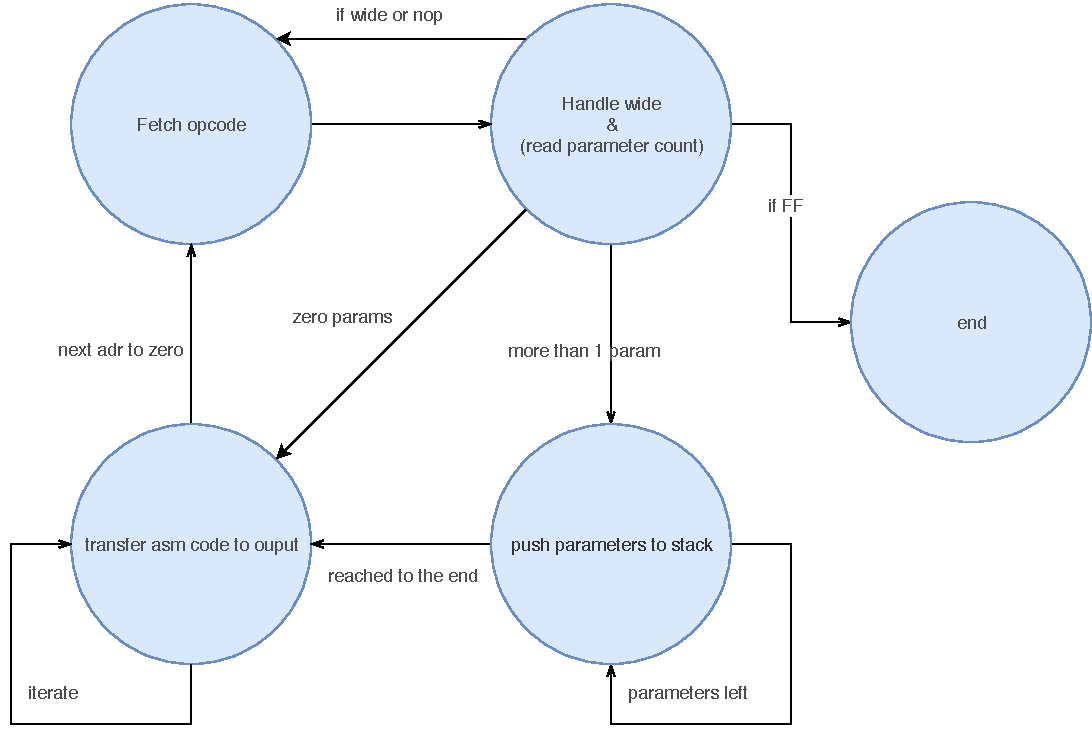
\includegraphics[width=0.9\linewidth]{SM}
	\caption{ماشین حالت}
	\label{fig:sm}
\end{figure}
%%% May add some information
\subsection*{\lr{FETCH\_INSTRUCTION}}
در این استیت، آپکد دستور 
\lr{JVM}،
 از رم مربوط به آن خوانده می‌شود. و بعد برای بررسی نوع دستور و گرفتن تعداد پارامترهای آن، به استیت (۲) می‌رویم. 

\subsection*{\lr{CHECK\_WIDE\_AND\_READ\_COUNTER}}

با بررسی آپکد دستور که در مرحله‌ی قبل خوانده‌ایم، در این‌جا با بررسی نوع دستور، به یکی از استیت‌های زیر می‌رویم:
\subsection*{\lr{END}}
برای پایان برنامه از یک بایت که در دستورات JVM نیست
\LTRfootnote{reserved word}
 مانند
\lr{0xFF}
استفاده کرده‌ایم. در صورتی که آپکد برابر این کلمه باشد، برنامه‌ی داخل رم JVM تمام شده‌است و کار این ماژول به پایان می‌رسد. 
\subsection*{ITERATE}
با استفاده از
\lr{count\_rom}
که همان‌طور که قبلاً توضیح داده شده‌است، ماژولی است که با توجه به آپکد دستورات JVM، تعداد بایت پارامترهایی که بعد از آن آپکد قرار می‌گیرند را مشخص می‌کند - می‌توان تعداد پارامترهای هر آپکد را در این‌جا داشت. بنابراین اگر پارامتری پس از این آپکد نداشته باشیم، مستقیماً به این استیت می‌رویم.